% !TEX root = tutor-2-10-3.tex
% Edit tasks in task-2-10-3.tex.
\def\TutorEdition{1}
\expandafter\def\csname TutorSource8AB566\endcsname{\href{https://ege.fipi.ru/bank/questions.php?search=1\&proj=BA1F39653304A5B041B656915DC36B38\&qid=8AB566}{Источник: 8AB566}}
\expandafter\def\csname TutorSourceA53641\endcsname{\href{https://ege.fipi.ru/bank/questions.php?search=1\&proj=BA1F39653304A5B041B656915DC36B38\&qid=A53641}{Источник: A53641}}
\expandafter\def\csname TutorSource35343\endcsname{\href{https://phys-ege.sdamgia.ru/problem?id=35343}{Источник: Решу ЕГЭ, №35343}}
\expandafter\def\csname TutorSource41579\endcsname{\href{https://phys-ege.sdamgia.ru/problem?id=41579}{Источник: Решу ЕГЭ, №41579}}
\expandafter\def\csname TutorSource3435\endcsname{\href{https://phys-ege.sdamgia.ru/problem?id=3435}{Источник: Решу ЕГЭ, №3435}}
\expandafter\def\csname TutorSource20038\endcsname{\href{https://phys-ege.sdamgia.ru/problem?id=20038}{Источник: Решу ЕГЭ, №20038}}
\expandafter\def\csname TutorSource50827\endcsname{\href{https://phys-ege.sdamgia.ru/problem?id=50827}{Источник: Решу ЕГЭ, №50827}}
\expandafter\def\csname TutorSource2988\endcsname{\href{https://phys-ege.sdamgia.ru/problem?id=2988}{Источник: Решу ЕГЭ, №2988}}
% !TEX root = task-2-10-3.tex
% Editable task bank. Append new BankTask blocks at the end of the document.
\documentclass[12pt,a4paper]{article}
\usepackage{physics-textbook}
\usepackage{graphicx,needspace}
\usetikzlibrary{decorations.pathmorphing}
\newif\ifShowSolutions
\ifdefined\TutorEdition
  \ShowSolutionstrue
\else
  \ShowSolutionsfalse % Change to \ShowSolutionstrue to display solutions.
\fi
\newcounter{banktask}
\newsavebox{\BankTaskBox}
\newcommand{\BankTaskContent}[3]{%
  \noindent\textbf{\thebanktask.}\quad #2\par
  \ifShowSolutions
    \Needspace{50mm}% Keep the solution heading with its opening text or diagram.
    #3\par
    \ifdefined\TutorEdition
      \ifcsname TutorSource#1\endcsname
        \nopagebreak\smallskip{\small\csname TutorSource#1\endcsname\par}%
      \fi
    \fi
  \fi
}
\newcommand{\BankTask}[3]{%
  \refstepcounter{banktask}\par\medskip
  \sbox{\BankTaskBox}{\begin{minipage}{\linewidth}%
    \BankTaskContent{#1}{#2}{#3}\end{minipage}}%
  \ifdim\dimexpr\ht\BankTaskBox+\dp\BankTaskBox\relax>\dimexpr\textheight-20mm\relax
    \Needspace{35mm}\BankTaskContent{#1}{#2}{#3}%
  \else
    \Needspace{\dimexpr\ht\BankTaskBox+\dp\BankTaskBox\relax}%
    \noindent\usebox{\BankTaskBox}\par
  \fi
  \medskip
}
\begin{document}
\BookSubsection{2.10.3}{Удельная теплота плавления}


% Source 8AB566: https://ege.fipi.ru/bank/questions.php?search=1&proj=BA1F39653304A5B041B656915DC36B38&qid=8AB566
\BankTask{8AB566}{
Какое количество теплоты необходимо для того, чтобы расплавить $2\,\text{кг}$ свинца, взятого при температуре плавления (в $\text{кДж}$)?
}{
\smallskip\noindent\textbf{Решение от GPT}\par
$Q=\lambda m=2{,}5\cdot10^4\cdot2=5\cdot10^4\,\text{Дж}=50\,\text{кДж}$. Ответ: $50\,\text{кДж}$.
}

% Source A53641: https://ege.fipi.ru/bank/questions.php?search=1&proj=BA1F39653304A5B041B656915DC36B38&qid=A53641
\BankTask{A53641}{
\begin{center}
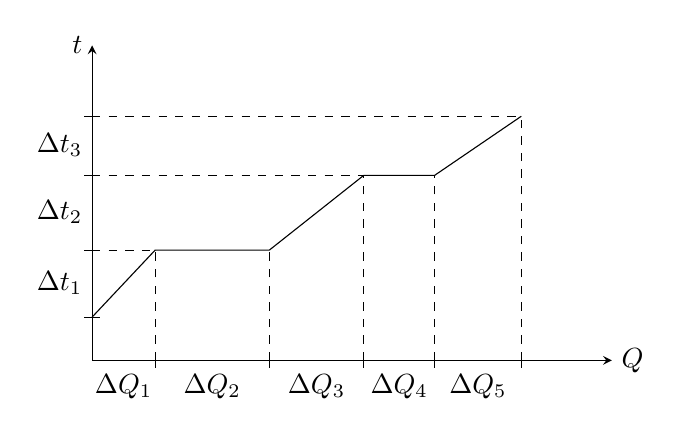
\begin{tikzpicture}[x=1cm,y=1cm,>=stealth]
\draw[->] (0,0)--(6.6,0) node[right] {$Q$};
\draw[->] (0,0)--(0,4) node[left] {$t$};
\draw (0,0.55)--(0.8,1.4)--(2.25,1.4)--(3.45,2.35)--(4.35,2.35)--(5.45,3.1);
\foreach \x/\y in {0.8/1.4,2.25/1.4,3.45/2.35,4.35/2.35,5.45/3.1} {
\draw[dashed] (\x,0)--(\x,\y);
\draw (\x,0.1)--(\x,-0.1);
}
\foreach \y in {0.55,1.4,2.35,3.1} {\draw (-0.1,\y)--(0.1,\y);}
\draw[dashed] (0,1.4)--(0.8,1.4);
\draw[dashed] (0,2.35)--(3.45,2.35);
\draw[dashed] (0,3.1)--(5.45,3.1);
\node[left] at (0,0.98) {$\Delta t_1$};
\node[left] at (0,1.88) {$\Delta t_2$};
\node[left] at (0,2.73) {$\Delta t_3$};
\node[below] at (0.4,-0.06) {$\Delta Q_1$};
\node[below] at (1.525,-0.06) {$\Delta Q_2$};
\node[below] at (2.85,-0.06) {$\Delta Q_3$};
\node[below] at (3.9,-0.06) {$\Delta Q_4$};
\node[below] at (4.9,-0.06) {$\Delta Q_5$};
\end{tikzpicture}
\end{center}
В цилиндре под поршнем находилось твёрдое вещество массой $m$. Цилиндр поместили в печь. На рисунке схематично показан график изменения температуры $t$ вещества по мере поглощения им количества теплоты $Q$. Формулы А и Б позволяют рассчитать значения физических величин, характеризующих происходящие с веществом тепловые процессы.

Установите соответствие между формулами и физическими величинами, значение которых можно рассчитать по этим формулам.



\begin{center}
\TaskMatchingColumns[.35\linewidth]{Формулы}{
А) $\displaystyle\frac{\Delta Q_1}{m\Delta t_1}$\par
Б) $\displaystyle\frac{\Delta Q_2}{m}$
}{Физические величины}{
1) удельная теплота плавления\par
2) удельная теплота парообразования\par
3) удельная теплоёмкость твёрдого вещества\par
4) удельная теплоёмкость жидкости
}

\begin{tabular}{|c|c|}
\hline
А & Б \\
\hline
\phantom{3} & \phantom{1} \\
\hline
\end{tabular}
\end{center}
}{
\smallskip\noindent\textbf{Решение от GPT}\par
А: первый наклонный участок соответствует нагреванию твёрдого вещества. Из $\Delta Q_1=mc_{\text{тв}}\Delta t_1$ получаем $c_{\text{тв}}=\dfrac{\Delta Q_1}{m\Delta t_1}$, поэтому А~--- 3.

Б: первый горизонтальный участок соответствует плавлению при постоянной температуре. Из $\Delta Q_2=\lambda m$ получаем $\lambda=\dfrac{\Delta Q_2}{m}$, поэтому Б~--- 1.

Ответ: $31$.
}

% Source 35343: https://phys-ege.sdamgia.ru/problem?id=35343
\BankTask{35343}{
В стакан калориметра, содержащий $250\,\text{г}$ воды, опустили кусок льда массой $140\,\text{г}$, имевшего температуру $0^\circ\text{C}$. После того как наступило тепловое равновесие, весь лед растаял, и температура воды стала равной $0^\circ\text{C}$. Определите начальную температуру воды. Теплоёмкостью калориметра
и теплообменом с окружающей средой пренебречь.
}{
\smallskip\noindent\textbf{Решение}\par
Поскольку потери по условию отсутствуют, то все количество теплоты, отданное водой при охлаждении от начальной температуры $t_1$ до температуры плавления
\[Q_1=m_{\text{в}}c(t_{\text{пл}}-t_1),\]
пошло на плавление льда
\[Q_2=m_{\text{л}}\lambda.\]
Запишем уравнение теплового баланса
\[Q_1+Q_2=0,\]
или
\[cm_{\text{в}}(t_1-t_2)=\lambda m_{\text{л}},\]
откуда
\[t_1=\frac{\lambda m_{\text{л}}}{cm_{\text{в}}}+t_2.\]
Подставив числовые значения, получим искомую величину:
\[t_1=\frac{3{,}3\cdot 10^5\cdot0{,}14}{4200\cdot0{,}25}+0=44^\circ\text{C}.\]
Ответ: $44^\circ\text{C}$.
}

% Source 41579: https://phys-ege.sdamgia.ru/problem?id=41579
\BankTask{41579}{
Кусок льда опустили в термос с водой массой $1100\,\text{г}$, имеющей начальную температуру $15 ^\circ\text{C} .$ Начальная температура льда равна $0 ^\circ\text{C} .$  При достижении теплового равновесия в воде остаётся плавать кусочек льда. Какая масса льда растаяла в процессе перехода к тепловому равновесию? Теплоёмкостью термоса можно пренебречь.
}{
\smallskip\noindent\textbf{Решение}\par
Так как начальная температура льда равна температуре плавления, а при достижении теплового равновесия в воде остаются плавать кусочки льда, то делаем вывод, что установившаяся температура в сосуде равна $0$ \ensuremath{{}^\circ}C. При охлаждении воды выделилось количество теплоты $Q_1=mc ( t_{\,\text{пл}} - t ) ,$ на плавление льда потребовалось количество теплоты $Q_2=\lambda m_1.$
Из уравнения теплового баланса $Q_1 + Q_2=0$ находим массу растаявшего льда

\[m_1= \frac{mc ( t - t_{\,\text{пл}} )}{\lambda} = \frac{4200 \cdot 1{,}1 \cdot 15}{3{,}3 \cdot 10 ^{5}} =0{,}21 \,\text{кг}=210\,\text{г}.\]

Ответ: $210\,\text{г}$.
}

% Source 3435: https://phys-ege.sdamgia.ru/problem?id=3435
\BankTask{3435}{
В теплоизолированный сосуд с большим количеством льда при температуре $t_1=0 ^\circ\,\text{С}$ заливают $m=1\,\text{кг}$ теплой воды. Какова была начальная температура воды, если при установлении теплового равновесия в сосуде расплавилось $560\,\text{г}$ льда? Ответ приведите в градусах цельсия.
}{
\smallskip\noindent\textbf{Решение}\par
При контакте тел с разной температурой, между ними начинается теплообмен. он продолжается до тех пор, пока температуры тел не выровняются. Льда в термосе много, а значит, весь лед не растает, и конечная температура системы будет $0 ^\circ\,\text{С}.$ Поскольку система находится в термосе, теплопотерями можно пренебречь. На плавление льда требуется количество теплоты $Q_1=\Delta m\lambda,$ при охлаждении воды выделяется количество теплоты $Q_2=cm ( t_1 - t_2 ) .$ 
Составим уравнение теплового баланса: 

$Q_1 + Q_2=0.$ 
$\Delta m\lambda + cm ( t_1 - t_2 ) =0.$ 

 В итоге для начальной температуры воды в сосуде с учетом, что $t_1=0 ^\circ C,$ получаем:

\[t_2= \frac{\lambda \Delta m}{cm} = \frac{3{,}3 \cdot 10 ^{ 5 } \cdot 0{,}56}{4200 \cdot 1} =44 ^\circ\,\text{С}.\]

Ответ: $44$ °C.
}

% Source 20038: https://phys-ege.sdamgia.ru/problem?id=20038
\BankTask{20038}{
В калориметре находятся в тепловом равновесии вода и лед. После опускания в калориметр болта, имеющего массу $165\,\text{г}$ и температуру –$40$ \ensuremath{{}^\circ}С, $20$\% воды превратилось в лед. Удельная теплоемкость материала болта равна $500\,\text{Дж}$/(кг · К). Какая масса воды первоначально находилась в калориметре? Теплоемкостью калориметра пренебречь.
}{
\smallskip\noindent\textbf{Решение}\par
Так как вода и лед находятся в тепловом равновесии, то и до опускания болта, и после его нагревания температура в сосуде $t_{0}$  =  $0$ \ensuremath{{}^\circ}С. Согласно уравнению теплового баланса количество теплоты, выделившееся при замерзании воды, было затрачено на нагревание болта: $0{,}2m \cdot r = cm_1 ( t_0 - t ) ,$ где m  — масса воды в сосуде, $m_{1}$  — масса болта, с  — удельная теплоемкость болта, r  — удельная теплота плавления льда, t  — начальная температура болта. Получим:

\[m= \frac{cm_1 ( t_0 - t )}{0{,}2r} = \frac{500 \cdot 0{,}165 \cdot 40}{0{,}2 \cdot 3{,}3 \cdot 10 ^{5}} =0{,}05 \,\text{кг}.\]

Ответ: m  =  $0{,}05\,\text{кг}$.
}

% Source 50827: https://phys-ege.sdamgia.ru/problem?id=50827
\BankTask{50827}{
В калориметре находится $1\,\text{кг}$ льда при температуре −$5$ °C. Какую массу воды, имеющей температуру $20$ °C, нужно добавить в калориметр, чтобы температура его содержимого после установления теплового равновесия оказалась −$2$ °C? Теплообменом с окружающей средой и теплоёмкостью калориметра пренебречь.
}{
\smallskip\noindent\textbf{Решение}\par
В результате теплообмена происходят процессы нагревания льда от $t_{1}$ до установившейся температуры t, охлаждение воды от $t_{2}$ до $t_{\,\text{пл}}=0 ^\circ \,\text{С},$ кристаллизация воды и охлаждение образовавшегося льда от $t_{\,\text{пл}}$ до установившейся температуры t. Для каждого из этих процессов запишем количество теплоты: 

$Q_1=m_1\,\text{с}_{\,\text{л}} ( t - t_1 ) ;$
$Q_2=m_2c_{\,\text{в}} ( t_{\,\text{пл}} - t_2 ) = - m_2c_{\,\text{в}}t_2;$
$Q_3= - \lambda m_2;$
$Q_4=m_2c_{\,\text{л}} ( t - t_{\,\text{пл}} ) =m_2c_{\,\text{л}}t.$

Так как при теплообмене отсутствует теплообмен с окружающей средой, то уравнение теплового баланса имеет вид:

$Q_1 + Q_2 + Q_3 + Q_4=0,$
$m_1\,\text{с}_{\,\text{л}} ( t - t_1 ) - m_2c_{\,\text{в}}t_2 - \lambda m_2 + m_2c_{\,\text{л}}t=0,$

откуда находим массу воды:

\[m_2= \frac{m_1\,\text{с}_{\,\text{л}} ( t - t_1 )}{c_{\,\text{в}}t_2 + \lambda - c_{\,\text{л}}t} = \frac{1 \cdot 2100 \cdot ( - 2 + 5 )}{4200 \cdot 20 + 330000 + 2100 \cdot 2} \approx 0{,}015\,\text{кг}=15\,\text{г}.\]

Ответ: $15\,\text{г}$.
}

% Source 2988: https://phys-ege.sdamgia.ru/problem?id=2988
\BankTask{2988}{
В калориметре находился лед при температуре $t_1= - 5 ^\circ\,\text{С}.$ Какой была масса $m_1$ льда, если после добавления в калориметр $m_2=4\,\text{кг}$ воды, имеющей температуру $t_2=20 ^\circ\,\text{С},$ и установления теплового равновесия температура содержимого калориметра оказалась равной $t=0 ^\circ\,\text{С},$ причем в калориметре была только вода?
}{
\smallskip\noindent\textbf{Решение}\par
Количество теплоты, полученное при нагреве льда, находящегося в калориметре, до температуры $t=0 ^\circ C$: $Q_1=c_1m_1 ( 0 - t_1 )$ ($1$).
Количество теплоты, полученное льдом при его таянии при $0 ^\circ\,\text{С}:$ $Q_2=\lambda m_1$ ($2$).
Количество теплоты, отданное водой при охлаждении ее до $0 ^\circ\,\text{С}:$ $Q=c_2m_2 ( t_2 - 0 )$ ($3$). 
Уравнение теплового баланса: $Q=Q_1 + Q_2$ ($4$). 
Объединяя ($1$)–($4$), получаем: 

\[m_1= \frac{m_2}{c} _2 ( t_2 - 0 ) c_1 ( 0 - t_1 ) + \lambda = \frac{4 \cdot 4200 \cdot 20}{2100 \cdot 5 + 3{,}3 \cdot 10 ^{5}} \approx 1\,\text{кг}.\]

Ответ: $m_1\approx 1\,\text{кг}.$
}

\end{document}

